\documentclass [12pt, a4paper, oneside, titlepage, ngerman]{article}
\usepackage{times}
\usepackage[ngerman]{babel} 
\usepackage[utf8]{inputenc}
\usepackage[T1]{fontenc} 
\usepackage[pdfborder={0 0 0}]{hyperref}
\usepackage{color}
\usepackage{graphicx}
\usepackage{float}
\usepackage{natbib}
\usepackage{enumitem}
\usepackage[printonlyused]{acronym}
\usepackage{url}
\usepackage{ltablex}
\usepackage{pdfpages}

\usepackage{geometry} \geometry{a4paper, top=25mm, left=20mm, right=40mm, bottom=20mm} 
\renewcommand{\baselinestretch}{1.5}

\begin {document}



\begin{titlepage}
\Large
\begin{minipage}{\textwidth} \centering \Large
     Duale Hochschule Baden-Württemberg \\  
     Mannheim 
\end{minipage} \vspace{1cm}

\begin{minipage}{\textwidth} \centering \Large
     \textbf{Erste Projektarbeit \\ Erarbeitung eines Lösungsentwurfes für eine IT-Lösung zur Kapazitätsplanung der Kabinencrew}
\end{minipage} \vspace{1cm}

\begin{minipage}{\textwidth} \centering \Large
     \mbox{Studiengang Wirtschaftsinformatik - Sales \& Consulting}\\  \large Bearbeitungszeitraum: 15.05.2017 - 29.08.2017
\end{minipage} \vspace{1cm}


\begin{table}[h!]
\begin{tabular}{ll}
Verfasser: & Julian Garske \\
Matrikelnummer: & 6728241 \vspace{0.5cm} \\ 
Kurs: & WWI SCA16 \\
Studiengangsleiter:& Prof. Dr. Frank Koslowski \vspace{0.5cm} \\
Wissenschaftlicher Betreuer: & Günter Stumpf \\ 
Telefon:& 01511 8237778\\ 
Mailadresse:& guenter.stumpf@esosec.de \vspace{0.5cm}\\
Ausbildungsbetrieb: &Lufthansa Systems GmbH \& Co. KG \\ 
& Am Prime Parc 1 \\ 
& D 65479 Raunheim \vspace{0.5cm}\\
Unternehmensbetreuer: & Iwan Berger \\ 
Telefon(Firma): &+49 (0)69 696 74135 \\
 Mailadresse(Firma):& iwan.berger@lhsystems.com \\
\end{tabular}
\end{table}



\end{titlepage}

\tableofcontents
\newpage


\pagenumbering{gobble}


\pagenumbering{Roman}
\section*{Abkürzungsverzeichnis}
\addcontentsline{toc}{section}{Abkürzungsverzeichnis}

\begin{acronym}[NL/C]

\acro{BT} {Beschäftigungstage}
\acro{CAB} {Compas Cabin}
\acro{CDB} {Crew Database}
\acro{CMS} {Crew Management System}
\acro{COC} {Compas Cockpit}
\acro{CP} {Captain}
\acro{FO} {First Officer}
\acro{KG} {Kleingruppe}
\acro{LSY} {Lufthansa Systems}
\acro{NL/C} {NetLine/Crew}
\acro{PU} {Planungseinheit}

\acro {SFO} {Senior First Officer}



\end{acronym}
\newpage


\addcontentsline{toc}{section}{Abbildungsverzeichnis}
\listoffigures
\newpage


\pagenumbering{arabic}
\setcounter{page}{1}
\section{Einleitung}
\subsection {Motivation}

Bereits seitdem es kommerzielle Passagierflüge gibt, ist eine konkrete Zuteilung der Besatzung für die Flüge notwendig. Dabei müssen nicht nur Fehlzeiten wie Urlaub oder Krankheit, sondern auch andere Faktoren wie z.B. Teilzeit berücksichtigt werden. Außerdem werden für unterschiedliche Flugzeuge auch unterschiedliche Qualifikationen benötigt. Bei immer größer werdenden Fluggesellschaften, wie der Lufthansa mit insgesamt ca. 20.000 Besatzungsmitgliedern der Kabine, stellt die mengenmäßige Einteilung der Kabinenbesatzung aus diesen Gründen oft eine Herausforderung dar. Die sogenannte Kapazitätsplanung ist deshalb für viele Airlines ein wichtiger Bestandteil des Flugbetriebs. \\
Mit der Kapazitätsplanung hängt die Schulungsplanung eng zusammen. Schulungen dauern oft einige Wochen und müssen daher langfristig vorher geplant werden, sodass Fehlzeiten ausgeglichen werden können und die Qualifikationen nach der Schulung aktualisiert werden. Das Ziel der Kapazitäts- und Schulungsplanung ist, "`durch rechtzeitige Neueinstellungen und Umschulungen die richtige Menge an Piloten mit der richtigen Qualifikation zum richtigen Zeitpunkt auf einer Flotte bereitzustellen"' \cite[vgl.][S.19]{compasdoku}. \\

\noindent Für die Kapazitäts- und Schulungsplanung der Cockpit-Besatzung im Lufthansa Konzern gibt es seit 2000 das von Lufthansa Systems entwickelte System COMPAS (Crew Operation Manpower Planning Advanced System), im folgenden \ac{COC} genannt. Dadurch ist eine Planung der Einteilung und Schulungen für die etwa 5.000 Piloten bis zu 15 Monate in Zukunft möglich. Bis heute wird die Funktionalität dieses Programms regelmäßig erweitert.  \\
Mit der Entwicklung von \ac{COC} entstand der Wunsch, ein ähnliches Programm auch für die Kabinenbesatzung zu entwickeln. Durch diese systematische Lösung sollen aufwendige manuelle Prozesse abgelöst und damit Zeit gespart und Fehler minimiert werden \cite[vgl.][S.4]{highlevelitems}. Ein Auftrag für das Projekt wurde von dem Kunden, der Lufthansa Passage Airline, noch nicht vergeben, weshalb es noch nicht zu einem Projekt mit einer konkreten Analyse oder Entwicklung kam.  \\

\noindent Im Jahr 2016 hatte sich die Firma M2P Consulting bereits mit der bisherigen Kapazitätsplanung der Kabinenbesatzung auseinandergesetzt und geprüft, wie man diese verbessern könne und ob \ac{COC} dafür in Frage käme. Sie kamen zu dem Ergebnis, dass kurzfristig zwar die bisherige Vorgehensweise der Kapazitätsplanung (siehe \ref{vorgehensweise}) optimiert werden könne, um die Qualität zu verbessern, langfristig solle es aber durch eine systemseitige Lösung abgelöst werden \cite [vgl.][S.8-10]{M2P}. %Formulierung?

\subsection {Problemstellung und -abgrenzung}
Zurzeit werden die mengenmäßigen Kapazitäten für die Einsätze der Kabinenbesatzung mithilfe von verschiedenen Excel-Tabellen geplant. Diese ca. 200 Tabellen enthalten Daten aus unterschiedlichen Quellen, die für die Zuteilung der Besatzung erforderlich sind. Aufgrund der großen Datenmenge und den Verflechtungen der Tabellen untereinander kommt es oft zu Problemen und Fehlern bei der Kapazitätsplanung \cite[vgl.][]{Gespraech2}. \\ 

\noindent Nach dem Vorbild von \ac{COC} soll eine automatisierte Kapazitäts- und Schulungsplanung jetzt auch für die Kabinenbesatzung unter dem Titel \ac{CAB} ermöglicht werden. Um den Umfang dieses Projektes einzugrenzen, wird mit der Kapazitätsplanung begonnen, die, sobald sie fertiggestellt wurde, um die Schulungsplanung ergänzt wird. Dabei gilt es, zu ermitteln wie weit \ac{COC} dafür als Vorlage genutzt werden kann, da dieses Tool den geforderten Zweck bereits für die Cockpitbesatzung erfüllt.\\
Im Vordergrund steht dabei zuerst die Anpassung der bereits vorhandenen Bestandsrechnung in \ac{COC} an die Kapazitätsplanung der Kabinenbesatzung. Diese informiert über den aktiven, verfügbaren Bestand an Piloten, indem von einem Ausgangswert, den "`brutto Beschäftigungsköpfen"', unterschiedliche An- und Abwesenheiten verrechnet werden. Die Bestandsrechnung ist die spätere Grundlage für die Kapazitätsplanung, in der sie mit dem Bedarf ins Verhältnis gesetzt wird, um ein Delta zu ermitteln, welches eine Über- oder Unterdeckung in Beschäftigungstagen anzeigt.\\ %ggf. später ergänzen, je nachdem wie weit wir kommenls Ausgangspunkt für das Projekt wird \ac{COC} genutzt, da es viele gewünschten Funktionen schon für die Cockpit-Besatzung enthält. Einige Unterschiede, die es zwischen der Kapazitätsplanung der Cockpit- und der der Kabinenbesatzung gibt, müssen analysiert und geklärt werden, um zu entscheiden, ob das gewünschte Programm in \ac{COC} integriert werden kann. Diese Unterschiede werden im Kapitel \ref{unterschiede} genauer erläutert. %Der Berechnungsalgorithmus soll nach der Behebung der Probleme ähnlich wie in \ac{COC} angewendet werden können. 
\\

%\noindent Besonderer Fokus liegt auf der Integration in die bestehende Systemlandschaft von \ac{COC} und die Entwicklung einer mandantenfähigen Lösung, um mehrere Airlines der Lufthansa Gruppe zu integrieren. Trotz der Integration soll das Programm mit Blick auf die Zukunft moderne Architekturansätze beinhalten und sich vom fast 20 Jahre alten Design von \ac{COC} loslösen.
%Darüberhinaus sollten die Berechnungsläufe getrennt von \ac{COC} erfolgen, um sich gegenseitig nicht zu beeinträchtigen \cite[vgl. dazu][]{anwenderkonzept}.

\subsection {Ziel der Arbeit} 
%Das Ziel dieser Projektarbeit ist, einen initialen Lösungsentwurf für die Entwicklung eines explorativen Prototyps zur Kapazitätsplanung des Kabinenpersonals zu erstellen. Daraus sollen vor allem die Anforderungen und Funktionen erkennbar sein. Der explorative Prototyp soll nach seiner Entwicklung evolutionär genutzt werden und damit Ausgangspunkt für Erweiterungen sein. \\
%Auf der Grundlage des Prototyps soll die sogenannte Deltarechnung ermöglicht werden. Dabei wird der aktuelle Personenbestand mit dem Bedarf ins Verhältnis gesetzt und damit die Kapazitäten ermittelt. Für zukünftige Prognosen werden Prämissen und Erfahrungswerte genutzt. \\

%\noindent In dieser Arbeit wird für die Kapazitätsplanung die Bestandsrechnung erläutert und angepasst. Darüber hinaus wird evaluiert, ob und wie weit \ac{COC} dazu als Vorlage dienen kann und welche Unterschiede in der Bestandsrechnung zwischen der Cockpit- und der Kabinenbesatzung beachtet werden müssen. Für Probleme, die aus diesen Unterschieden resultieren, soll eine Lösung gefunden werden, damit das Modell von \ac{COC} in ähnlicher Weise auf die Kapazitätsplanung der Kabine angewendet werden kann.
%NL/C fehlt noch, ggf. streichen

Zunächst war das Ziel der Arbeit, einen Lösungsentwurf für die Entwicklung eines Prototypes zur Kapazitätsplanung der Kabinenbesatzung zu erarbeiten. Darüber hinaus sollte diskutiert werden, wie weit \ac{COC} als Vorlage genutzt werden kann und welche Unterschiede es zur Kapazitätsplanung der Cockpitbesatzung gibt. \\
Relativ schnell wurde klar, dass der Aufwand, diesen Lösungsentwurf zu erarbeiten, den Umfang dieser Arbeit überschreitet. Das Hauptelement der Kapazitätsplanung ist die Deltarechnung, in der Bestand und Bedarf zueinander ins Verhältnis gesetzt werden und das Delta ermittelt wird. Besonders eine Lösung für die Automatisierung der Bedarfsrechnung der Kabinenbesatzung zu finden, in der für einen bestimmten Zeitraum der Bedarf an Flugpersonal der einzelnen Flotten ermittelt wird, stellte sich schnell als kompliziert heraus. Deswegen fokussiert sich diese Arbeit nur auf den ersten Schritt der Kapazitätsplanung, die Bestandsrechnung. \\
Während offiziell noch nicht entschieden wurde, ob das Programm ein Tool von \ac{COC} wird oder ob ein eigenständiges und moderneres Programm entwickelt wird, lässt sich bereits eine Tendenz erkennen. Die einfachste Lösung für alle Stakeholder ist, \ac{COC} als Vorbild zu nutzen, da es viele Gemeinsamkeiten mit dem gewünschten Programm bereits beinhaltet. Daher wird dieses ähnliche Tool in dieser Arbeit als Ausgangspunkt genutzt. \\
Diese Projektarbeit fokussiert sich damit auf die Unterschiede zwischen der Bestandsrechnung in \ac{COC} und der gewünschten automatisierten Bestandsrechnung für die Kabinenbesatzung. Es werden Lösungsansätze für Probleme, die aus erforderlichen Veränderungen entstehen, gefunden und beschrieben, wie \ac{COC} angepasst werden sollte, um eine automatisierte Bestandsrechnung für die Kabinenbesatzung zu ermöglichen.

\subsection {Vorgehen}
Zunächst ist es nötig, die Anforderungen zu ermitteln und abzuklären. Dafür muss zuerst die aktuelle Vorgehensweise der Kapazitätsplanung von der Cockpit- und der Kabinenbesatzung verstanden werden. Danach werden Anforderungen an die automatisierte Kapazitätsplanung der Kabinenbesatzung erfasst. Die Anforderungen werden in diesem Projekt hauptsächlich von den momentanen Planerinnen, die das spätere Programm anwenden, gestellt. \\
Danach werden Gemeinsamkeiten und Unterschiede zwischen \ac{CAB} und \ac{COC} ermittelt, um damit bewerten zu können, wie \ac{COC} als Vorlage geeignet ist. %Zwar könnten viele Dinge aus \ac{COC} für \ac{CAB} übernommen werden, jedoch soll im Gegenteil zu \ac{COC} ein modernes Programm entwickelt werden \cite[vgl.][]{Gespraech1}. \\ % Auch \ac{NL/C} wird dafür in Betracht gezogen. \\
Eine Anwenderdokumentation dient als Grundlage für die Entwicklung des Prototyps. Sie beschreibt aus fachlicher Sicht, wie Nutzer mit dem Programm interagieren und welche Funktionen es beinhaltet.

\subsection{Überblick über COMPAS Cockpit}
\ac{COC} (Crew Operation Manpower Planning Advanced System) dient als Ausgangspunkt für das Projekt und nur einige Besonderheiten müssen bei dem aktuellen Programms angepasst werden, um die Kapazitätsplanung der Kabinenbesatzung dadurch zu automatisieren \cite[vgl.][]{Gespraech1}. Deshalb sind ein Überblick über \ac{COC} und Kenntnisse der wichtigsten Funktionen davon wichtig. Dieser Überblick stammt aus einem betriebsinternen Dokument \cite[vgl.][]{compasdoku}. \\
\ac{COC} ist das zentrale Tool für die Kapazitätsplanung des Cockpitpersonals. Ziel dieser Planung ist es, die richtige Anzahl an Piloten mit passenden Qualifikationen zu einem bestimmten Zeitpunkt auf eine Flotte bereitstellen zu können. Das kann kurzfristig gesteuert oder langfristig prognostiziert werden. Diese Planung ist sehr komplex, da sehr viele Einflussfaktoren dort berücksichtigt werden müssen. \\
Um während der Planung den Überblick zu behalten, teilt \ac{COC} jeden Piloten eindeutig in eine \ac{PU} ein, die durch Flugzeugtyp, Flotte, Fluggesellschaft, Standort, Funktion und Unterfunktion definiert ist. Dadurch kann für jede \ac{PU} für einen bestimmten Zeitraum tagesgenau z.B. der Bestand und Bedarf ermittelt und verglichen werden. \\

\noindent \ac{COC} besteht nach einigen Erweiterungen mittlerweile aus folgenden drei Hauptmodulen:
\begin{itemize}
\item Deltarechnung: Setzt Pilotenbestand und -bedarf ins Verhältnis zueinander
\item Schulungsplan: Planung und Einteilung von Schulungskursen
\item Reportfunktionen: Detailabfragen bestimmter Daten
\end{itemize}

\noindent Als Zusatzmodule kommen Schnittstellen zu der COMPAS Datenbank und zu dem Bewerbersystem für das Cockpit hinzu \cite[vgl.][S.19]{compasdoku}.


\subsection{Bisherige Vorgehensweise der Kapazitätsplanung für die Kabinenbesatzung} \label{vorgehensweise}
Bisher gibt es für die Kapazitätsplanung der Kabine noch kein spezialisiertes Tool. Zwei Angestellte der Lufthansa Passage planen die Kapazitäten mithilfe von Excel-Tabellen. Dafür verknüpfen sie ca. 220 Tabellen miteinander \cite[vgl.][]{Gespraech2}. Da es kaum möglich ist, jede einzelne Person konkret einzuteilen, wird jede einer \ac{KG} zugewiesen. Diese werden ähnlich wie die \acp{PU} durch Funktion, Homebase, Unterfunktion, Fluggesellschaft und ein oder mehreren Flugzeugtypen definiert. Auf Grundlage dieser \acp{KG} wird die Kapazitätsplanung durchgeführt und nur bei Bedarf können einzelne Personen genauer betrachtet werden.  \\
Nach M2P Consulting sei "`die Handlungsfähigkeit der Kapazitätsplanung in Bezug auf die zukünftige Herausforderungen stark eingeschränkt"' \cite[S.5]{M2P} und "`deckt keine der definierten Soll-Funktionalitäten der Kapazitätsplanung ausreichend ab"' \cite[S.6]{M2P}. Bei den Soll-Funktionalitäten handelt es sich nach M2P um langfristige Bereederung und Budgetplanung und um mittelfristige Bereederung \cite[vgl.][S.6]{M2P}.

\newpage

\section{Problemanalyse} \label{unterschiede}
\subsection{Erhebung der Pilotendaten von der Crew Database} \label{cdberhebung}
Im Vergleich zu \ac{COC}, welches mit Daten von etwa 6.000 Piloten umgeht, muss \ac{CAB} in der Lage sein, Daten von etwa 20.000 Personen ohne große Schwierigkeiten verarbeiten zu können \cite[vgl.][]{Gespraech1}. Um diese Daten aktuell zu halten, werden alle zwei Wochen Quelldaten vorbereitet, was bereits in \ac{COC} einige Stunden dauert, für \ac{CAB} wäre es also bei einer linearen Steigung fast das Vierfache. Es besteht dabei jedoch das Risiko, dass die Laufzeit sogar exponentiell ansteigt. Bei einer langen Laufzeit erhöht sich zudem auch die Fehleranfälligkeit, da Abstürze wahrscheinlicher werden. \\
Hinzu kommt, dass die Datenbank nicht lange von \ac{CAB} ausgelastet werden darf, weil auch andere Schnittstellen darauf zugreifen. Eine zu starke Auslastung kann dabei zu großen Problemen in unterschiedlichen Bereichen und Systemen bei der Lufthansa Passage führen \cite[vgl.][]{Gespraech1}. \\

\noindent Bei der Erhebung der Daten in \ac{COC} werden von der \ac{CDB}, der zentralen Datenbank, alle benötigten Daten herausgesucht und daraus neue Views erstellt, sodass die Daten tagesgenau für die nächsten 450 Tage vorliegen. Dieses Erstellen der Views wird in dieser Arbeit auch Datenaufbereitung genannt. Daraus entstehen drei Tabellen. Sie enthalten Bestandsdaten sowohl für jede Person (personenbasiert) als auch für jede PU (kumuliert) und Stammdaten jedes Mitarbeiters, die für die Kapazitätsplanung benötigt werden. Die hohe Anzahl an Datensätzen führt dazu, dass die Tabellen der Views bis zu drei Millionen Einträge enthalten, die alle von der \ac{CDB} aufbereitet werden \cite[vgl.][]{Gespraech3}.  \\

\noindent Aus diesem Problem resultiert, dass für die Datenaufbereitung der \ac{CDB} eine neue Architektur benötigt wird, um das fast 20 Jahre alte Design von \ac{COC} abzulösen \cite[vgl.][]{Gespraech3}. Für eine Veränderung des Architekturansatzes zur Datenaufbereitung wird ein grobes Verständnis der bisherigen Architektur von \ac{COC} benötigt.

\subsection{Integration in das COMPAS-Umfeld}
Sobald \ac{CAB} weit genug entwickelt worden ist, soll es, den aktuellen Anforderungen nach, in das bereits bestehende \ac{COC} integriert werden. Der Kunde möchte momentan kein weiteres Programm haben. %Dabei soll eine Auswahl des Programms möglich sein und \ac{CAB} soll als Modul oder Erweiterung von \ac{COC} genutzt werden können \cite[vgl.][S.6]{anwenderkonzept}. 
Im Gegensatz dazu soll aber auch ein modernes Programm entwickelt werden. Deshalb ist es unklar, ob man dieses im Endeffekt in \ac{COC} integriert oder doch ein neues Programm entwickelt, was sogar als Vorlage für eine Modernisierung von \ac{COC} genutzt werden kann. Das Ergebnis dieses Projektes soll auch als Entscheidungshilfe dienen.\\



\subsection{Erfassen der Anforderungen} \label{anforderungen}
Bei der Anforderungsermittlung geht es darum, die vollständige und korrekte Anforderungen von den Stakeholdern zu ermitteln. In diesem Projekt werden die Anforderungen größtenteils von den Kabinenplanerinnen gestellt, dem sogenannten Fachbereich. \\

\noindent Herausforderungen bei der Ermittlung sind unterschiedliche und häufig wechselnde Anforderungen. Die Stakeholder können sie oft selber nicht genau benennen und ausdrücken, sodass die Wünsche sich zu widersprechen scheinen oder durch neue Ideen und Vorschläge ändern. %vgl. Zube
Ein anderer problematischer Teil ist das Sprachverständnis während der Anforderungsermittlung. Der "`Fachbereich [kennt] in den seltensten Fällen die Fachbegriffe des Entwicklers [...] und umgekehrt [...]. Somit ist eine Art 'Übersetzungsprozess' zwischen der Sprache des Fachbereichs und der des Entwicklers notwendig"' \cite[S.319]{Alpar2016} . 
Für den Auftragnehmer bedeutet das eine ständige Hinterfragung aller Details und Fachbegriffe sowie die Absprache jeder Kleinigkeit mit den Stakeholdern, sodass sie vollständig ihren Anforderungen entsprechen. \\



\subsection{Mehrfachqualifikationen der Kabinenbesatzung}
Jede Person der Kabinenbesatzung kann mehreren Flotten zugeordnet sein. Eine Person wird zwar genau einer \ac{KG} zugeteilt, aber diese \ac{KG} kann bis zu drei, aber auch weniger Flugzeugtypen haben, für die die zugeordneten Flugbegleiter und -begleiterinnen qualifiziert sind \cite[vgl.][]{Gespraech2}. \\
Auch in \ac {COC} ist die Zuteilung jeder Person zu einer \ac{PU} eindeutig. Jede \ac{PU} wird aber, im Gegensatz zu der Kabinenbesatzung, durch einen eindeutigen Flugzeugtypen definiert. Da die \acp{PU} Basis für die Berechnungen sind, basiert \ac{COC} auf der Tatsache, dass eine Person, anders als die Kabinenbesatzung, in genau einer Rolle auf genau einer Flotte fliegt. Deshalb muss das gewünschte Tool sinnvoll mit den Mehrfachqualifikationen der Kabinenbesatzung umgehen können. \\
Eine Übersicht aktueller \acp{KG} und \acp{PU} befindet sich im \autoref{kgpu}.

\newpage

\section {Grundlagen/Methodischer Ansatz}
\subsection{Der Software-Lebenszyklus}
Software Projekte lassen sich in einzelne Phasen unterteilen. Diese "`Phasen, die ein Softwareprodukt bei seiner Herstellung und dem späteren Einsatz durchläuft"' \cite[S.173]{gabler} nennt man den Software-Lebenszyklus eines Produktes.
\begin{figure}[H]
	\centering
	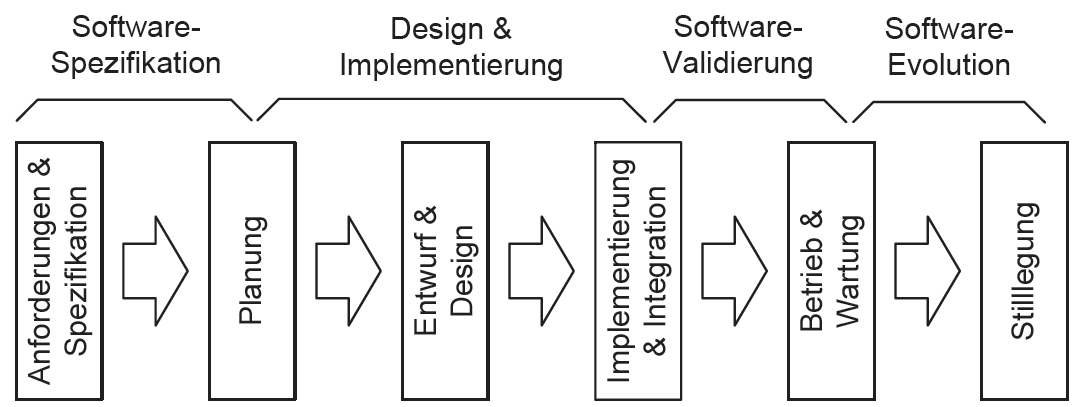
\includegraphics[width=\textwidth,keepaspectratio]{softwarelebenszyklus.PNG}
	\caption{Lebenszyklus eines Softwareprojekts}
	\cite[S.13]{schatten2010}
	\label{img:softwarelebenszyklus}
\end{figure}
\noindent In Abbildung \ref{img:softwarelebenszyklus} lassen sich die wesentlichen Schritte des Software-Lebenszyklus erkennen. Diese sind hier entweder grob in vier Stufen oder differenzierter in sechs Stufen unterteilt. Es gibt keine Festlegung über die Anzahl oder die Bezeichnungen der Abstufungen, sodass es sehr viele unterschiedliche Versionen des Software-Lebenszyklus und damit Vorgehensmodelle für die Softwareentwicklung gibt. Grundlegende Dinge, die hier durch \textit{Software-Spezifikation}, \textit{Design und Implementierung}, \textit{Software-Validierung} und S\textit{oftware-Evolution} dargestellt werden, "`finden sich [jedoch] nahezu in allen Projekten wieder"' \cite[S.13]{schatten2010}. \\ 
Detaillierter lässt sich der Software-Lebenszyklus in die sechs Phasen \textit{Anforderung und Spezifikation}, \textit{Planung}, \textit{Entwurf und Design}, \textit{Implementierung und Integration}, \textit{Betrieb und Wartung} und \textit{Stilllegung} aufteilen. \\
Die Einteilung eines Softwareprojekts in Phasen "`kann den Entwicklerteams als Leitlinie dienen, um ein Software-Projekt im Team erfolgreich zu strukturieren und abzuwickeln"' \cite[S.11]{schatten2010}. Dabei können die Phasen je nach Vorgehensmodell variieren oder wahrgenommen werden.


\subsection{Vorgehen bei der Beschreibung und Analyse der Anforderungen}
Die Beschreibung und Analyse von Anforderungen ist der erste Schritt bei fast jedem IT-Projekt. Zunächst wird "`aus der in einer systematischen Ermittlung gewonnenen Information [...] bei der Dokumentation eine präzise Anforderungsspezifikation erstellt"' \cite[S.44]{partsch2010}. In diesem Fall wird in Zusammenarbeit mit dem Kunden eine Anwenderdokumentation erstellt, die die Anforderungen beschreibt. Diese Anwenderdokumentation dient als Pflichtenheft und enthält "`die vom Auftragnehmer erarbeiteten Realisierungsvorgaben"' \cite[S.41]{PohlRupp2015}.\\
Statt dem Lastenheft werden für die Erstellung der Anwenderdokumentation nur mündliche Quellen genutzt, da es sich in diesem Fall um einen Entwurf für die Entwicklung eines Prototyps handelt. Mit dessen Hilfe soll es dem Nutzer vereinfacht werden, ein Lastenheft für die Entwicklung des endgültigen Programms zu erstellen. Anders als gewöhlich wird in diesem Projekt also eine Art Pflichtenheft mit einem Realisierungsvorschlag vom Auftragnehmer geliefert und danach erst das Lastenheft erstellt. Der Auftraggeber formuliert dann darin, wie weit er mit dem Lösungsvorschlag, also dem Prototypen, einverstanden ist und welche Änderungen und Ergänzungen benötigt werden. \\

\noindent Das Ziel der Anforderungsanalyse ist, "`möglichst vollständige Kundenanforderungen in guter Qualität zu dokumentieren und dabei Fehler möglichst frühzeitig zu erkennen und zu beheben"' \cite[S.11]{PohlRupp2015}. Dafür gibt es unterschiedliche Methoden, die jedoch alle "`vor allem gesunden Menschenverstand voraus[setzen]"' \cite[S.58]{partsch2010}.\\
Quelle zur Ermittlung der Anforderungen sind Dokumente, bereits existierende Systeme und hauptsächlich die sog. Stakeholder. Diese sind "`Person[en] oder Organisation[en], die (direkt oder indirekt) Einfluss auf die Anforderungen ha[ben]"'\cite[S.21]{PohlRupp2015}. Gemeint sind damit also alle Menschen, die in irgendeiner Weise mit der Software zu tun haben oder haben werden, z.B. der Kunde, der Nutzer, die Entwickler etc. \\
Da der Auftraggeber oft nicht in der Lage ist genau auszudrücken, was er will und braucht, ist es die Aufgabe des Requirement Engineers "`in Software-Projekten frühzeitig mit dem Kunden und den späteren Nutzern [zu] reden, um zu erfahren, was sie sich vorstellen"' \cite[S.15]{kleuker2006}.\\
Es muss also eine ständige Kommunikation und Zusammenarbeit sichergestellt werden. So eine Zusammenarbeit setzt "`ein gewisses Verständnis der Arbeitsabläufe des Kunden, genauer dessen Geschäftsprozesse \cite[vgl.][]{Gad03}, [voraus], die mit der zu entwickelnden Software im Zusammenhang stehen"' \cite[S.15]{kleuker2006}.


\subsection{Qualitätssicherung der Anforderungen}
"`Grundsätzlich gilt, dass die Produkte aller Tätigkeiten bei der Softwareentwicklung [...] qualitätsgesichert [...] werden müssen"' \cite[S.55]{Winter1999}. Deshalb "`ist es notwendig, die Qualität der [...] Anforderungen zu überprüfen"' \cite[S.95]{PohlRupp2015}, um Probleme der Anforderungsermittlung (siehe Kapitel \ref{anforderungen}) zu lösen.  \\
Diese ständige Qualitätssicherung dient dazu, Fehler möglichst früh innerhalb des Softwarelebenszyklus zu erkennen und zu beheben. Der Grund dafür ist, dass die Fehlerbehebung in der Softwareentwicklung mit steigendem Projektfortschritt mehr Aufwand verursacht \cite[vgl.][S.2]{hussmann}. Aufwand kann dabei Geld, Zeit oder auch andere zu erbringende Leistung oder Einsatz sein. Das Ziel ist daher, Fehler schon möglichst früh in dem Projektverlauf zu beseitigen. \\

\noindent Dieser Aufwand der Fehlerbehebung ist der Grund für die Qualitätssicherung der Anforderungsermittlung und dadurch ist sie so wichtig für den Erfolg eines Projektes. Diese wichtige Rolle wird in dem folgenden Balkendiagramm dargestellt:
\begin{figure}[H]
	\hspace{-2cm}
	\centering
	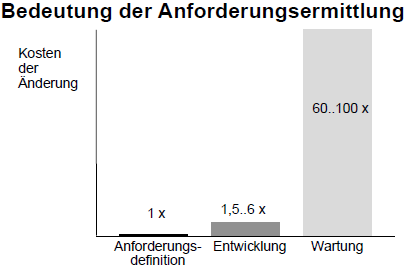
\includegraphics[width=350px,keepaspectratio]{TUDresden.png}
	\caption{Aufwand der Fehlerbehebung in Softwareprojekten}
	\cite[S.2]{hussmann}
	\label{img:TUDresden}
\end{figure}
\noindent Das Diagramm in der Abbildung beschreibt den Aufwand der Fehlerbehebung in einem Softwareprojekt in Abhängigkeit von dem Projektfortschritt. Dieser Fortschritt wird dabei in den drei Kategorien Anforderungsdefinition, Entwicklung und Wartung angegeben, die Abschnitte in fast jedem Software-Lebenszyklus sind. \\

\noindent Wird ein Fehler in der Phase der Anforderungsermittlung oder am Anfang des Projektes behoben, wird der Aufwand dafür mit dem Faktor Eins multipliziert. Sobald ein Fehler gefunden wurde, gilt es die Anforderung zu überarbeiten und ihn einfach zu korrigieren.\\
Während der Entwicklung des Projektes ist der Aufwand meist um das 1,5 bis 6-fache höher. Grund dafür ist, dass Fehler, die sich dann noch in der Software befinden, oft mehrere Bereiche betreffen und viel verändert und berücksichtigt werden muss bevor man sie endgültig beheben kann.\\
Am meisten Aufwand verursacht die Fehlerbehebung, falls der Fehler erst am Ende des Software-Lebenszyklus entdeckt wird. Dabei ist die Software schon in Betrieb und befindet sich in der Wartung. Um dort einen Fehler zu beheben, müssen oft ganze Programmabschnitte verändert werden, damit die Software wieder fehlerfrei läuft. Es hat also große Folgen, wenn ein Teil des Programmes während der Wartung verändert werden muss, weshalb der Aufwand etwa 60 bis 100 mal höher ist als zu Anfang des Projekts. \\
Deshalb ist es so wichtig, die einzelnen Phasen eines Software-Lebenszyklus sorgfältig zu bearbeiten und zu überprüfen, sodass keine Fehler auftreten oder diese schon so früh wie möglich erkannt werden. Es sollte daher nicht zu früh und unvorbereitet mit der Entwicklung begonnen werden. Andernfalls entsteht ein "Wegwerf-Prototyp", der "`kein Ersatz für die Dokumentation und auch kein brauchbarer Bestandteil des finalen Systems"' \cite[]{Kuhrmann2012} und damit nicht Ziel dieses Projektes ist.\\
Obwohl es Ausnahmen gibt, lohnt sich der Aufwand in der Analyse meistens, da "`viele schwerwiegende Fehler in den frühen Phasen IS-Entwicklung [Informationssystem-Entwicklung; Anmerk. d. Verf.] gemacht werden"' \cite[S.316]{Alpar2016}. Trotzdem wird in vielen Fällen zu voreilig mit der Entwicklung angefangen. \\
"Die Analyse der in einer Anforderungsdefinition festgelegten Anforderungen zielt letztlich darauf ab, Aufschluss über die Qualität der Anforderungsbeschreibung zu erhalten"' \cite[S.51]{partsch2010}. Kriterien für die Qualität lassen sich hauptsächlich in Inhalt, Dokumentation und Abgestimmtheit gliedern. Es wird sich also damit befasst, ob die Anforderungen vollständig, detailliert, passend dokumentiert und mit allen Stakeholdern abgestimmt sind. Für jeden der drei Qualitätsaspekte gibt es damit unterschiedliche Prüfkriterien \cite[vgl.][S.97]{PohlRupp2015}.

\subsubsection{Qualitätsaspekt Inhalt}
"`Der Qualitätsaspekt >>Inhalt<< bezieht sich auf die Überprüfung von Anforderungen auf inhaltliche Fehler"' \cite[S.98]{PohlRupp2015}. Dafür gibt es acht Prüfkriterien\cite[vgl.][S.98]{PohlRupp2015}: 
\begin{description}[font=\itshape]\setlength\itemsep{0em}
\item[Vollständigkeit:] Wurden alle relevanten Anforderungen erfasst?
\item[Korrektheit:] Beschreibt jede Anforderung die dafür notwendigen Informationen?
\item[Verfolgbarkeit:] Können die Anforderungen verfolgt, also z.B. auf die Quelle zurückgeführt werden?
\item[Adäquatheit:] Enthalten die Anforderungen die Bedürfnisse und Wünsche der Stakeholder angemessen?
\item[Konsistenz:] Gibt es Widersprüche zwischen den Anforderungen?
\item[Vorzeitige Entwurfsentscheidungen:] Wurden Entwurfsentscheidungen vorweggenommen, die nicht durch Randbedingungen bestimmt sind?
\item[Überprüfbarkeit:] Können Abnahme- und Prüfkriterien anhand der Anforderungen definiert werden?
\item[Notwendigkeit:] Trägt jede Anforderung zu dem definierten Ziel bei?
\end{description}

\subsubsection{Qualitätsaspekt Dokumentation}
Bei der Dokumentation geht es darum, die "`Anforderungen auf Mängel in der Dokumentation bzw. auf Verstöße gegen geltende Dokumentationsvorschriften"'\cite[S.99]{PohlRupp2015} zu überprüfen. Hierbei gibt es folgende vier Prüfkriterien\cite[vgl.][S.99f.]{PohlRupp2015}:
\begin{description}[font=\itshape]\setlength\itemsep{0em}
\item[Konformität:] Wurden die Anforderungen in dem vorgeschriebenen Dokumentationsformat strukturiert und in der richtigen Modellierungssprache dokumentiert?
\item[Verständlichkeit:] Können die Anforderungen in dem gegebenen Kontext ggf. mithilfe eines Glossars verstanden werden?
\item[Eindeutigkeit:] Ist eine eindeutige Interpretation möglich?
\item[Konformität mit Dokumentationsregeln:] Sind vorgegebene Dokumentationsregeln und -richtlinien eingehalten worden?
\end{description}

\subsubsection{Qualitätsaspekt Abgestimmtheit}
Die Abgestimmtheit stellt sicher, dass keine "'Mängel in der Abstimmung der Anforderungen unter relevanten Stakeholdern"'\cite[S.100]{PohlRupp2015} vorliegen. Auch dafür gibt es folgende drei Prüfkriterien\cite[vgl.][S.100]{PohlRupp2015} :
\begin{description}[font=\itshape]\setlength\itemsep{0em}
\item[Abstimmung:] Wurde jede Anforderung mit relevanten Stakeholdern abgestimmt?
\item[Abstimmung nach Änderungen:] Wurde jede Änderung der Anforderungen auch abgestimmt?
\item[Konflikte:] Wurden alle bekannten Konflikte gelöst?
\end{description}

\subsection{Anforderungskategorisierung}
Anforderungen werden kategorisiert und nach Wichtigkeit eingeteilt. Das ist hilfreich, da die Anforderungen unterschiedlich zur Zufriedenheit der Stakeholder beitragen \cite[vgl.][S.24]{PohlRupp2015}. Durch Kategorisierung lassen sie sich leichter einordnen, um Aufwand und Priorität besser abschätzen zu können. \\
In diesem Fall werden die Anforderungen nach dem Kano-Modell kategorisiert. Demnach gibt es drei Kategorien \cite[vgl. S.24]{PohlRupp2015}:
\begin{description} 
\item[Basisfaktoren] sind selbstverständliche unterbewusste Systemmerkmale, die vorausgesetzt werden. 
\item[Leistungsfaktoren] sind bewusste, explizit geforderte Systemmerkmale.
\item[Begeisterungsfaktoren] sind für den Stakeholder unbekannte Systemmerkmale, die er während der Benutzung als angenehme Überraschung entdeckt.
\end{description}
Mit der Zeit werden aus Begeisterungsfaktoren Leistungsfaktoren und aus Leistungsfaktoren Basisfaktoren, da der Nutzer sich an die Merkmale gewöhnt und sie irgendwann voraussetzt. Das Modell lässt sich grafisch darstellen: 

\begin{figure}[H]
	\centering
	\includegraphics{kano.pdf}
	\caption{Grafische Darstellung des Kano-Modells}
	\cite[S.25]{PohlRupp2015}
	\label{img:kano}
\end{figure}
\noindent Die Grafik zeigt die Zufriedenheit der Stakeholder in Abhängigkeit von dem Erfüllungsgrad der jeweiligen Faktoren. Auf einer dritten Achse wird die Zeit dargestellt, wodurch die Anforderungen die Kategorien wechseln können. \\
Die Basisfaktoren müssen erfüllt sein, um eine massive Unzufriedenheit der Stakeholder zu vermeiden \cite[vgl. S.106]{Kano}. Sie werden vorausgesetzt und haben daher nur den Nutzen, Unzufriedenheit zu vermeiden. Daher verläuft die Funktion negativ exponentiell. \\
Die Funktion der Leistungsfaktoren verläuft linear und schneidet den Nullpunkt. Diese Faktoren erzeugen proportional Unzufriedenheit, wenn sie nicht erfüllt sind, und Zufriedenheit, wenn sie erfüllt sind \cite[vgl. S.106]{Kano}. \\
Da die Begeisterungsfaktoren vorher den Stakeholdern nicht bekannt sind und damit nicht erwartet werden können, kann ihr unzureichender Erfüllungsgrad keine Unzufriedenheit verursachen \cite[vgl. S.106]{Kano}. Das Vorhandensein dieser Faktoren freut jedoch die Stakeholder, wodurch es zu einem überproportionalen Nutzen bei steigender Erfüllung kommt. Deshalb ist die Funktion der Begeisterungsfaktoren exponentiell und erreicht niemals den Wert null oder weniger, aber steigt sehr schnell an. \\

\noindent Es ist ungeklärt, ob man diese Faktoren und ihre Eigenschaften so auf die Anforderungen bei der Erstellung eines Prototyps anwenden kann. Laut Pombergers Definition soll ein explorativer Prototyp ermöglichen, die Vorstellungen der Anwender "`anhand von Anwendungsbeispielen zu prüfen und die gewünschte Funktionalität zu ermitteln"' \cite[S.27]{pomberger2004}, er soll also die Analyse und die Anforderungsspezifikation unterstützen. Das bedeutet, dass der Prototyp nicht alle Anforderungen enthalten kann, besonders die Leistungs- und Begeisterungsfaktoren nicht, und genau im Gegenteil dazu dient, Anforderungen zu ermitteln. \\
Kanos Begeisterungsfaktoren widersprechen zudem dem weit verbreiteten Vorgehen bei einer erfolgreichen Anforderungsanalyse. Wie von Pohl und Rupp beschrieben ist dafür "`eine gute Kommunikation und [...] Qualität der Zusammenarbeit mit den Stakeholdern"' \cite[S.33]{PohlRupp2015} notwendig, um ihn "`erfolgreich in den Ermittlungsprozess einzubinden"' \cite[S.34]{PohlRupp2015}. Durch diese enge Zusammenarbeit werden alle Anforderungen abgesprochen, sodass es theoretisch kaum noch Begeisterungsfaktoren geben kann.


\subsection{Abgrenzung des Systems und Systemkontextes}
Die Abgrenzung eines Systems zu seiner Umgebung und zu den Schnittstellen ist essentiell für den Entwurf eines korrekten Produktes. Dafür müssen die System- und Kontextgrenzen bestimmt werden. \\
Dadurch wird Aufwand vermieden, indem bereits vorhandene Funktionen evtl. integriert oder nur in etwas veränderter Weise übernommen werden. Außerdem bringt sie Klarheit über die Arten der Informationsgewinnung und -weiterverarbeitung, um Missverständnisse zu vermeiden. Es ist wichtig, "`die Grenzen des Systems zum Systemkontext und die Grenzen des Systemkontexts zur irrelevanten Umgebung zu bestimmen"' \cite[S.20]{PohlRupp2015}, da der Systemkontext "`auch die Anforderungen an das zu entwickelnde System bestimmt"' \cite[S.20]{PohlRupp2015}. \\
Da diese Arbeit \ac{COC} als Grundlage nutzt sind auch die Systemgrenzen und -schnittstellen ähnlich. Wie bereits beschrieben muss nur die Schnittstelle zur \ac{CDB} etwas verändert werden. Nach der Erarbeitung des Lösungsentwurfs ist es dann die Entscheidung des Kunden, ob \ac{CAB} in \ac{COC} eingegliedert werden soll und die Abgrenzung damit größtenteils wegfällt oder ob System und Systemkontext für ein neues Programm neu bestimmt werden müssen.

\subsection{Arten und Ziele des Prototypings}
Prototyping beschreibt "`eine Vorgehensweise bei der Softwareentwicklung, bei der nicht sofort ein endgültiges Softwaresystem, sondern zunächst ein oder mehrere Prototypen erstellt werden"' \cite[S.152]{gabler}. Dabei wird nach Kuhrmann zwischen horizontalem und vertikalem Prototyping unterschieden \cite[vgl.][]{Kuhrmann2012}: \\ 
\textbf{Horizontales Prototyping} bezieht sich auf einen bestimmten Bereich der Software, z.B. die Benutzeroberfläche. Der Bezug zu der technischen Funktionalität und der tatsächlichen Implementierung ist dabei nicht gegeben. Nur die eine Ebene des Programms soll vorgestellt werden.\\
Beim \textbf{vertikalen Prototyping} wird ein Ausschnitt komplett in allen Ebenen vollständig implementiert. Diese Art dient zur Demonstration von komplexer Funktionalität.\\

\noindent Darüber hinaus unterscheidet die IEEE das Prototyping anhand von Anwendungszwecken \cite[vgl.][S.826]{ieeeprot}: 
\begin{description}
\item[Exploratives Prototyping] wird benutzt, wenn man das Problem und die Anforderungen noch nicht genau kennt. Indem viele Ideen und Ansätze ausprobiert werden, lernt der Entwickler die Arbeit und die Anforderungen des Kunden besser kennen, um die Anforderungen zu identifizieren.
\item[Experimentelles Prototyping] zielt auf das Sammeln von Erfahrungen und Ideen. Der Anwender kann mit dem Prototypen experimentieren, um Ideen an das Programm weiterzuentwickeln und Anforderungen zu konkretisieren. Währenddessen enthält der Entwickler Eindrücke von der Realisierbarkeit des Systems und technischen Herausforderungen.
\item[Evolutionäres Prototyping] stellt die Softwareentwicklung nicht als ein temporäres Projekt, sondern als eine fortlaufende Entwicklung dar. Dabei wird das Programm nach und nach erweitert, wobei der Entwickler eng an der Seite des Anwenders das System immer weiter erweitert.
\end{description}
Die Definition des evolutionären Prototypings widerspricht jedoch der allgemeinen Definition nach \cite{gabler}. Das Ergebnis des explorativen und des experimentellen Prototypings ist ein Prototyp im engeren Sinne, der der Demonstration dient. Dieser wird nach der Erfüllung seiner Aufgaben nicht mehr benötigt \cite[vgl.][S.21]{liggesmeyer2012}. Beim evolutionären Prototyping hingegen entsteht ein Pilotsystem, das der Kern des Produktes ist. Der Prototyp wird also fließend zum laufenden Produkt \cite[vgl.][S.24]{liggesmeyer2012} und ist damit eigentlich kein Prototyp laut Definition mehr, sondern schon ein endgültiges Softwaresystem.

\newpage

\section {Istanalyse}

\subsection{Bestandsrechnung in COMPAS Cockpit} \label{bestandsrechnung}
Der aktuelle Algorithmus für die Bestandsrechnung in \ac{COC} ermittelt zuerst den Bruttobestand der Besatzungen \cite[vgl.][S.8]{capfunc}. Die Einheiten für alle Bestands- und Bedarfsrechnungen sind verfügbare \ac{BT} oder Stunden. \\
Der Bestand wird ermittelt, indem der aktuelle Pilotenbestand mit allen Formen von Zu- und Abgängen z.B. durch Umschulungen, Altersabgänge, Neueinstellungen oder Kündigungen sowie allen bezahlungswirksamen Fehlzeiten wie Teilzeit, Mutterschutz oder Fluguntauglichkeit errechnet wird \cite[vgl.][S.19]{benutzerhandbuch}. Insgesamt gibt es 16 Kategorien, die hier aber der Übersicht halber nicht alle genannt werden. \\
Von diesem Bruttobestand werden alle weiteren Fehlzeiten, die sich grob in Urlaub und Krankheit einteilen lassen, subtrahiert, was zu dem Nettobestand führt \cite[vgl.][S.8]{capfunc}. \\
Das Ergebnis aller verfügbaren Piloten ergibt sich dann durch die Subtraktion von freien Tagen, die den Piloten zustehen. Auch die Arten und die Berechnung der freien Tage werden hier nicht weiter erläutert. \\
Dadurch ergibt sich der Bestand aller verfügbaren Piloten in \acp{BT}. Diese \acp{BT} lassen sich auf Tages-, Wochen- und Monatsbasis darstellen und zusammenfassen. Ein Screenshot der Bestandsrechnung aus \ac{COC} befindet sich im \autoref{bestandscreen}, wo weitere Details erkennbar sind.


\subsection{Anforderungsanalyse- und kategorisierung}
Die Planerinnen formulierten folgende Anforderungen \cite[vgl.][]{Gespraech2}:
\begin{description}
\item Basisfaktoren: Es soll ein Programm erstellt werden, dass die Kapazitäts- und später auch die Schulungsplanung automatisch regelt. Dafür müssen vor allem die Gruppen und Untergruppen eingeteilt und dargestellt werden können. Der Zeitraum soll 15 Monate betragen, um die Urlaubsplanung des jeweils kommenden Jahres mit einfließen lassen zu können. Eine Bestandsrechnung wird also benötigt, die später um die Bedarfsrechnung ergänzt werden soll. Wird eine Integration in das COMPAS-Umfeld beschlossen, wird das Programm nach und nach erweitert bis es in etwa den Funktionalitäten von \ac{COC} entspricht. \\
Der Kunde legt außerdem viel Wert auf Nachvollziehbarkeit. Es soll bei jeder Zelle der Tabellen verstanden werden können, woher die Daten kommen oder wie sie berechnet werden. Dazu soll es wie bei \ac{COC} die Möglichkeit geben, sich einzelne Detailabfragen anzeigen lassen zu können.
\item Leistungsfaktoren: Da es sich um den Entwurf eines Prototyps zur Kapazitätsplanung handelt, ist die Bedarfsrechnung und die Schulungsplanung ein Leistungsfaktor. Dazu gehören auch Bewerbungen für Schulungen. Diese Leistungsfaktoren werden aber später ergänzt, sodass sie nicht Bestandteil dieses Lösungsentwurfs sind. \\
Darüber hinaus wird eine gute Performance erwartet, um die Planung zu erleichtern und Zeit zu sparen.
\item Begeisterungsfaktoren: Modernes Design ist einer der Begeisterungsfaktoren. Dabei ist wünschenswert, das Programm so zu designen, dass sich Cockpit- und Kabinenplaner/innen ersetzen können und die Bedienung und Anordnung der Elemente gleich ist. 
\end{description}
Da sich diese Arbeit aber nur mit der Entwicklung eines Lösungsentwurfs für den Prototypen beschäftigt, stehen die Basisfaktoren im Vordergrund. Die Leistungs- und Begeisterungsfaktoren sind in einem explorativen Prototypen noch nicht vorhanden. Sie kommen im Verlauf des Projektes dazu. Trotzdem ist eine Bestimmung davon wichtig, Kernfunktionen des Systems festzulegen und Schwerpunkte festzulegen.

\subsection {Die Schnittstelle: Das Crew Management System}
Die Quelle, aus der \ac{COC} die benötigten Daten entnimmt, ist die \ac{CDB}, welche Bestandteil des \ac{CMS} ist. Unter dem \ac{CMS} wird das gesamte Planungssystem der Lufthansa verstanden, das aus vielen verschiedenen einzelnen Systemen, wie eine Crew Einsatzplanung oder einer Umlaufplanung, besteht. Im Mittelpunkt davon steht die \ac{CDB}, in der Daten zusammen fließen und in einer Datenbank gespeichert werden. Es wird also von mehreren unterschiedlichen Systemen aus auf die \ac{CDB} zugegriffen. Diese gleichzeitigen Lese- und Schreibzugriffe mehrerer Systeme müssen in kurzer Zeit von der \ac{CDB} bearbeitet werden können.\\
Nachdem die Daten in der \ac{CDB}, wie in Kapitel \ref{cdberhebung} beschrieben, aufbereitet wurden, werden die daraus entstandenen Views in die eigene COMPAS-Datenbank geladen, auf die \ac{COC} zugreifen kann. 
%Wenn über \ac{COC} die aktuellen Daten angefordert werden, werden sie in die eigene COMPAS-Datenbank geladen, wo direkt drauf zugegriffen werden kann. Das Aktualisieren der Tabellen aus der Views nimmt dabei nicht viel Zeit in Anspruch, da die Daten nur geladen und nicht verändert oder formatiert werden müssen.

\newpage
\section [Konkrete Modernisierung und Anpassung von COMPAS Cockpit]{Konkrete Modernisierung und Anpassung von \\ Compas Cockpit}
\subsection{Veränderungen bei der Datenaufbereitung}
Um Laufzeit- und Performanceprobleme bei der Datenaufbereitung zu vermeiden, wird eine andere Vorgehensweise als in \ac{COC} benötigt. Die einfachste Möglichkeit dazu ist, alle Rohdaten, aus denen die Views erstellt werden, unverändert von der \ac{CDB} in den eigenen Teil der Datenbank von \ac{COC} zu laden. Dort werden die Views erstellt von einem für \ac{COC} dedizierten Server erstellt und dem Tool weitergegeben \cite[vgl. dazu][]{Gespraech5}. \\
Dadurch hat die \ac{CDB} nur noch die Aufgabe, die Tabellen der Rohdaten zur Verfügung zu stellen, und es wird ihr keine große Leistung abverlangt. Die Auslastung wird von der \ac{CDB} auf den COMPAS-eigenen Server verschoben. Weil \ac{COC} diesen Server nur nutzt, um kurzzeitige zyklische Aufgaben auszuführen, ist es kein Problem, diesen für eine längere Dauer auszulasten. Selbst bei starker Auslastung wird damit kein anderes System beeinträchtigt. Durch eine höhere Programmiersprache und einem effizienteren Algorithmus kann die Datenaufbereitung möglicherweise deutlich schneller erfolgen. Nach der Erstellung der Views werden alle daraus erhaltenen Daten wie bislang wieder in den COMPAS-eigenen Teil der \ac{CDB} geladen, worauf das Programm darauf zugreift. \\

\noindent Bei der Datenaufbereitung wird mit personenbezogenen Daten gearbeitet, weshalb beim Erstellen der Views "`die Bestimmungen des Bundesdatenschutzgesetzes"' \cite[S.6]{CMS} und weitere "`spezielle Schutzvorschriften [,die] zwischen den Geschäftsleitungen und den Mitarbeitervertretungen [der Lufthansa AG; Anmerk. d. Verf.] definiert [wurden]"' \cite[S.6]{CMS}, gelten. Obwohl für beide Systeme die gleichen Sicherheitsvorkehrungen gelten, musste diese Vorgehensweise diskutiert und eine Genehmigung benötigt werden. 

\subsection{Veränderungen in der Bestandsrechnung} %oder doch ganz anders?
In der in Kapitel \ref{bestandsrechnung} beschriebenen Bestandsrechnung von \ac{COC} müssen einige Zeilen angepasst werden, damit sie der bisherigen Bestandsrechnung der Kabine entspricht. Diese Anpassungen wurden mit dem Kunden detailliert besprochen \cite[vgl.][]{bestanddet}. \\
Einige Zeilen wie "`Verlängerer Teilzeit"' oder "`Alterssonderurlaub"' fallen weg, da so etwas bei der Kabinenbesatzung nicht vorkommen kann. Eine Änderung wird für das Feld "`Umschulungen"' benötigt, das in \ac{COC} aus der bereits implementierten Schulungsplanung berechnet wurde. In \ac{CAB} ist es notwendig, zwischen Schulungen, die kürzer als fünf Tage, und welchen, die mindestens fünf Tage dauern zu unterscheiden, weshalb zwei Zeilen für eine mauelle Eingabe beider Arten benötigt werden. \\ %Wieso?
Bei der restlichen Bestandsrechnung kann genau so vorgegangen werden, wie es bereits in \ac{COC} für die Cockpit-Mitarbeiter implementiert ist.

%\subsection{Prämissen der Bestandsrechnung}

\subsection{Abbilden der Mehrfachqualifikationen und Einbindung der Kleingruppen} %TODO
Nach Absprache mit dem Kunden über das Problem der Mehrfachqualifikationen wurde dafür folgender Lösungsansatz gefunden \cite[vgl.][]{Gespraech4}: \\
Es soll die Möglichkeit geben, die \acp{KG} manuell \acp{PU} zuzuordnen. Die \acp{KG} sind auf der \ac{CDB} definiert und verfügbar, weshalb sie nicht vom Nutzer bearbeitet werden können. Es soll für ihn aber möglich sein, \acp{PU} anzulegen, zu bearbeiten und zu entfernen. Jede \ac{KG} wird dann vom Nutzer genau einer \ac{PU} zugeordnet. \\
Deshalb ist eine Verbindung zwischen einer Person und einer \ac{PU} nur über die \ac{KG} möglich, der sowohl die Person als auch die \ac{PU} zugewiesen ist. Jede Person wird also anstatt einer \ac{PU} mit einer \ac{KG} verknüpft. Danach ist eine neue Tabelle notwendig, in der die \acp{KG} den \acp{PU} zugeordnet werden, welche vom Anwender bearbeitet werden kann. Die Mehrfachqualifikationen fließen somit in das Konzept der \acp{PU} ein und es kann für jede \ac{PU} der Bestand ermittelt werden. Eine eindeutige Bedarfsrechnung ist mit dieser Methode aber noch nicht möglich. \\
%Lösung wie die Qualifikationen in die PUs einfließen

\newpage

\section {Zusammenfassung und Ausblick}
\subsection{Änderungen an COMPAS Cockpit um es für eine automatisierte Kapazitätsplanung der Kabinenbesatzung zu nutzen}
Um auf Grundlage von \ac{COC} die Kapazitätsplanung der Kabinenbesatzung zu automatisieren, müssten einige Dinge des Programms angepasst werden: \\
Die Funktionsweise der Datenaufbereitung muss aufgrund der höheren Anzahl an Quelldaten und ihrer Aufbereitung verändert werden. Eine nahe liegende Lösung dafür ist, die Datenaufbereitung von der \ac{CDB} auf einen anderen Server zu verlegen, der nur von \ac{COC} genutzt wird. Dazu kann der Algorithmus durch Nutzung spezieller Programmier-Bibliotheken verbessert werden. \\
Um Mehrfachqualifikationen der Kabinenbesatzung für Flotten sinnvoll in das Programm mit aufzunehmen, werden die \acp{KG}, die die Qualifikationen enthalten vom Nutzer selbst \acp{PU} zugewiesen. Dadurch ist eine eindeutige Bestandsrechnung möglich. Die Bestandsrechnung an sich ist für die Kapazitätsplanung der Cockpit- und der Kabinenbesatzung nahezu dieselbe. \\
Des Weiteren ist es nötig, viele Kleinigkeiten, z.B. Datenfelder oder Prämissen für eine Prognosenberechnung, anzupassen und detailliert mit dem Kunden abzustimmen. Daraus ergibt sich, welche Funktionen nicht mehr oder zusätzlich benötigt werden. Die hauptsächlichen Funktionen bleiben aber im Vergleich zu \ac{COC} unverändert. \\
Durch die Ähnlichkeit der Kapazitätsplanung in beiden Bereichen, ist es relativ einfach, \ac{CAB} in \ac{COC} einzugliedern und es als Vorlage zu nutzen. Mithilfe der in dieser Arbeit gefundenen Lösungsansätzen sollte es keine großen Schwierigkeiten mehr beinhalten, die Bestandsrechnung der Kabinenbesatzung zu automatisieren. \\
Das ursprüngliche Ziel, einen Lösungsentwurf für die gesamte Kapazitätsplanung der Kabinenbesatzung zu erstellen, wurde nicht erreicht, der hier entworfene Lösungsansatz für die Bestandsrechnung dient aber als Grundlage dafür.

\subsection{Probleme bei der Anpassung der Bedarfsrechnung der Kabinenbesatzung nach dem Vorbild von COMPAS Cockpit}
Nachdem die Bestandsrechnung relativ einfach angepasst werden kann, um den Bestand des Kabinenpersonals zu ermitteln, entstehen bei der Anpassung der Bedarfsrechnung weitere Probleme. Der Bedarf wird als nächster Schritt benötigt, um aus Bestand und Bedarf die Kapazität als Differenz zu ermitteln. Bekommt die Lufthansa ein neues Flugzeug, beispielsweise einen Airbus A340, wird für dieses Flugzeug eine Cockpitbesatzung benötigt. Dieser Bedarf fällt auf eindeutige \acp{PU} zurück, die genau die Piloten beinhalten, die in den benötigten Funktionen eine A340 fliegen. Da jede \ac{PU} des Cockpits eindeutig ist, kann der Bedarf einfach zugeordnet werden. \\
Aufgrund der Mehrfachqualifikationen entstehen bei der Bedarfszuordnung der Kabinenbesatzung aber Schwierigkeiten. Für die Kabinenbesatzung gibt es für eine Rolle z.B. eine \ac{PU}1, in denen die Leute auf einer A380 und einer A340 fliegen, aber auch eine \ac{PU}2, in denen sie auf A340 und Boeing 747 eingeteilt sind. Entsteht nun ein Bedarf an Kabinenpersonal für eine A340 ist es unklar, ob dieser aus \ac{PU}1 oder \ac{PU}2 abgedeckt wird. \\
Ein erster Lösungsansatz wäre es, den Bedarf prozentual auf alle möglichen \acp{PU} zu verteilen und diese zu gewichten. Wie genau damit umgegangen wird, muss aber mit dem Kunden ausführlich diskutiert werden, damit man sich auf eine Lösung einig wird.


\subsection{COMPAS Cockpit als Vorlage - kritische Auseinandersetzung}
Kurzfristig gesehen ist die Integration in \ac{COC} eine Lösung, mit der man mit wenig Aufwand das gewünschte Ziel, eine automatisierte Kapazitätsplanung der Kabinenbesatzung, erreichen kann.\\
Dieser Lösungsansatz ist jedoch kaum nachhaltig. \ac{COC} ist technisch gesehen auf einem fast 20 Jahre alten Stand. Gerade in der IT-Branche, die sich sehr schnell weiterentwickelt, ist dies eine sehr lange Zeit. Für die Gegenwart reicht es bis jetzt noch, aber in einigen Jahren können sich die Anforderungen an ein modernes, komplexes Programm und seinen Funktionen so stark verändern, dass das alte \ac{COC} dafür nicht mehr ausreicht. Deshalb wäre es vergeudeter Aufwand, den einfachen Weg zu gehen, um in einigen Jahren trotzdem ein fast komplett neues und modernes Programm zu entwickeln, wenn festgestellt wird, dass die Grenzen von \ac{CAB} überschreitet werden. \\
Es sollte lieber jetzt Aufwand in ein neues, eigenständiges und modernes Programm investiert werden; früher oder später reicht die bisherige Lösung nicht mehr aus und doppelte Arbeit bleibt dadurch erspart. Außerdem könnte \ac{CAB} vielleicht auch ein Vorbild für eine Modernisierung von \ac{COC} sein. Es ist im Sinne der Lufthansa, langfristig die beste Lösung in allen Bereichen zu finden, um auch in Zukunft ein einflussreiches und erfolgreiches Unternehmen zu bleiben.

\subsection{Weitere Vorgehensweise}
Zunächst müssen Probleme und Unterschiede bei der Bedarfsrechnung diskutiert und geklärt werden. Sobald es eine Lösung gibt, diese anzupassen, kann auf Grundlage darauf die Deltarechnung erstellt werden. Das entspricht dem gröbsten Teil der Kapazitätsplanung. Hinzu kommen noch Detailabfragen und Prämissen, die abgesprochen werden müssen, bevor die Kapazitätsplanung nach Vorbild von \ac{COC} in einem Prototypen implementiert werden kann. Als nächstes wäre es sinnvoll, eine automatisierte Lösung für die Schulungsplanung der Kabinenbesatzung zu entwickeln. \\
Der Prototyp dient als Entscheidungshilfe, um die wahrscheinlich wichtigste Anforderung zu klären. Die Stakeholder können sich damit vor Augen führen, wie gut \ac{COC} als Vorbild für die Kapazitätsplanung der Kabinenbesatzung geeignet ist. Sie müssen dann entscheiden, ob sie diese in \ac{COC} integrieren oder in ein größeres Projekt investieren, um eine komplett neue Software zu entwickeln.

\newpage

\pagenumbering{gobble}
\addcontentsline{toc}{section}{Literaturverzeichnis}
\bibliographystyle{natdin}

\bibliography{literatur}


\newpage

\pagenumbering{Roman}
\setcounter{page}{3}
\section* {Glossar}
\addcontentsline{toc}{section}{Glossar}


\begin{tabularx}{\textwidth}{l|X}
\textbf{Begriff} & \textbf{Erläuterung} \\\hline
Bestandsrechnung & Berechnung des verfügbaren Bestands in Beschäftigungstagen; dieser wird aus dem Bruttobestand und verschiedenen Ab- und Zugängen errechnet\\
COMPAS Cabin & Gefordertes Programm; soll in COMPAS Cockpit integriert werden und die Kapazitäts- und Schulungsplanung der Kabinencrew automatisieren\\
COMPAS Cockpit & Crew Operation Manpower Planning Advanced System; Programm zur Kapazitäts- und Schulungsplanung der Cockpit-Mitarbeiter: für die Lufthansa Passage von Lufthansa Systems 1999 entwickelt und seitdem ständig erweitert\\
Crew Database & Zentrale Datenbank der Lufthansa mit Schnittstellen zu vielen unterschiedlichen Systemen; stellt die erforderlichen Daten für COMPAS zusammen\\
Crew Management System & Überbegriff für alle Schnittstellen-Systeme der Lufthansa mit der Crew Database im Mittelpunkt\\
Deltarechnung & Der Bestand wird ins Verhältnis zum Bedarf gesetzt und daraus das Delta ermittelt\\
Funktion & auch Function; Rolle und Aufgaben, die Piloten oder die Kabinenbesatzung auf einem Flug übernehmen \\
Homebase & auch Standort; Flughafen an dem eine Person oder Gruppe stationiert ist \\  
IEEE & Institute of Electrical and Electronics Engineers; Berufsverband von Igenieuren aus Elektro- und Informationstechnik \\
Kapazitätsplanung & Mithilfe der Deltarechnung sollen dabei die richtige Anzahl an Personen mit den richtigen Qualifikationen zum richtigen Zeitpunkt verfügbar sein\\
Kleingruppe & Gruppen für die Kap.- und Schulungsplanung der Kabinenebesatzung; definiert durch  Funktion, Homebase, Unterfunktion, Fluggesellschaft und Flugzeugtyp(en)\\
Planungseinheit & auch Planningunit; Gruppen für die Kap.- und Schulungsplanung des Cockpits; definiert durch Flugzeugtyp, Funktion, Homebase, Fluggesellschaft, Unterfunktion\\
Unterfunktion & auch Subfunction; optionale Erweiterung der Funktion \\

\end{tabularx}

\newpage

\setcounter{page}{4}
\section* {Anhang}
\addcontentsline{toc}{section}{Anhang}
\appendix
\addtocontents{toc}{\protect\setcounter{tocdepth}{-1}}
\section{\mbox{Detaillierte Bestandsrechnung in COC - Screenshot}} 
\label{bestandscreen}
\begin{flushleft}
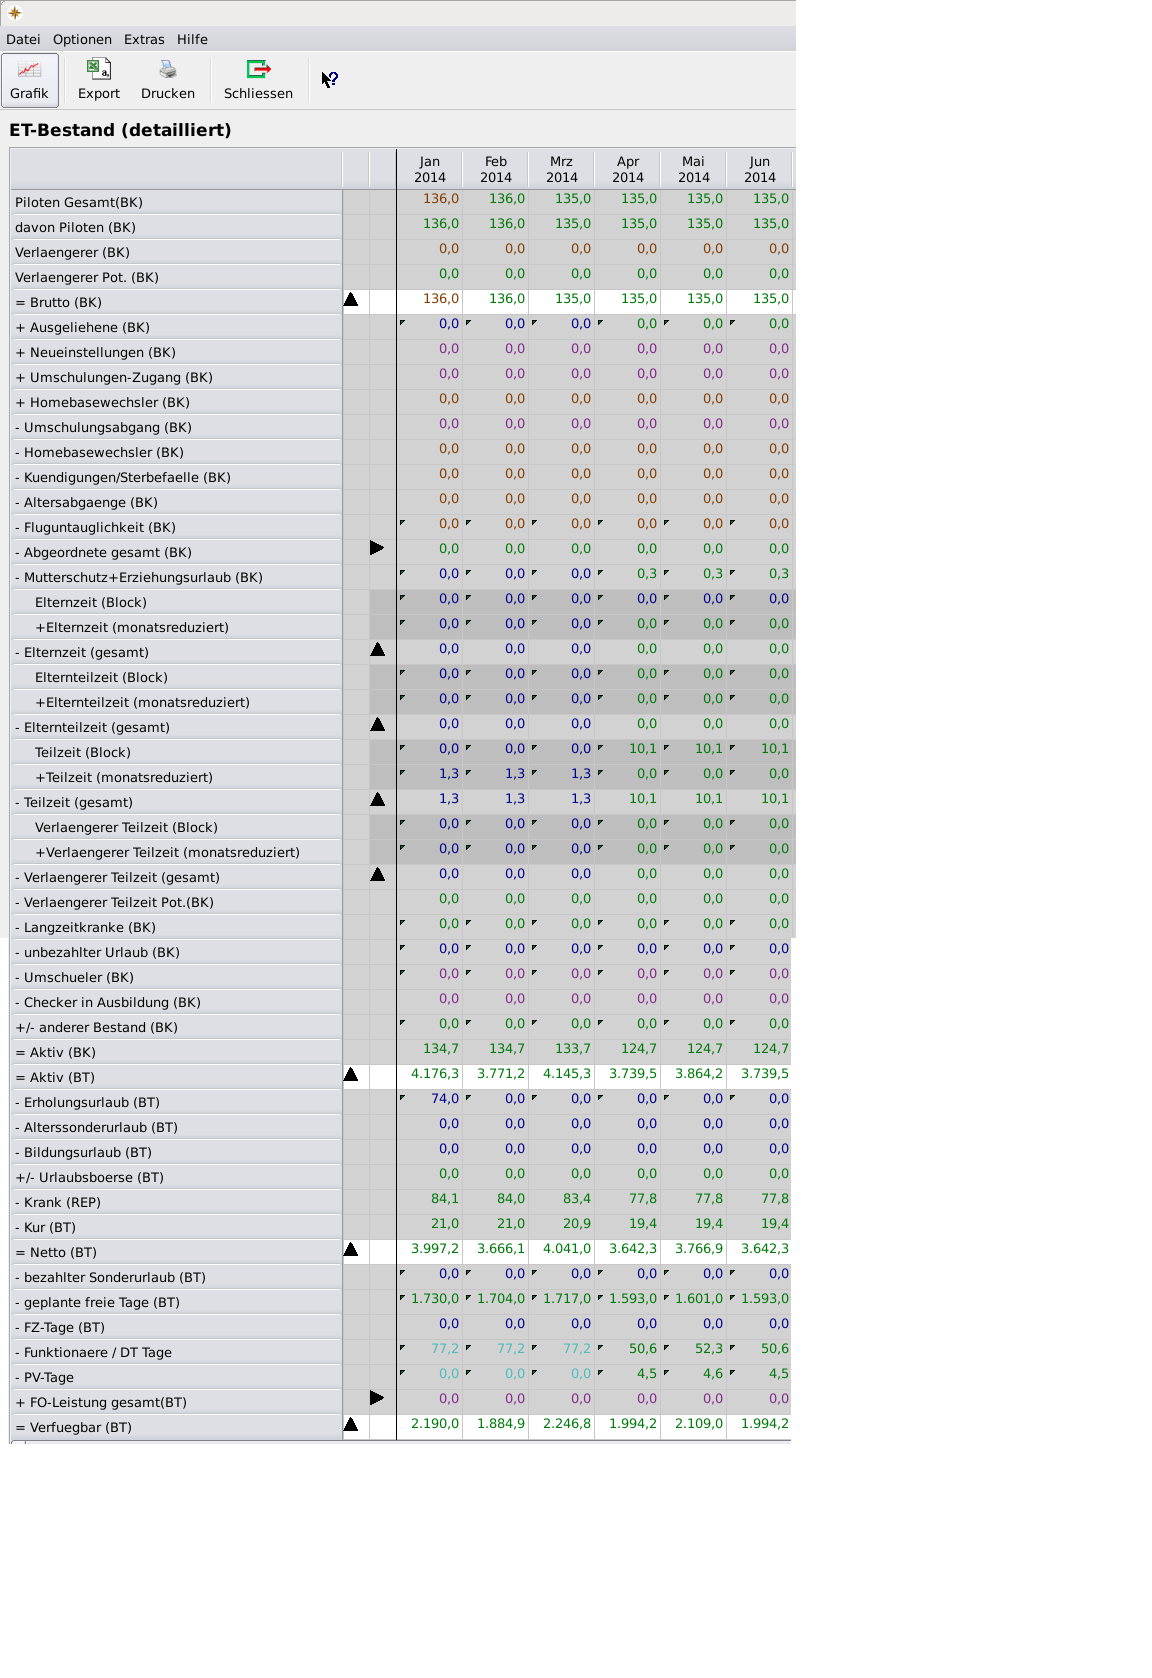
\includegraphics[width = 500px, keepaspectratio]{Bestand.png}
\end{flushleft}

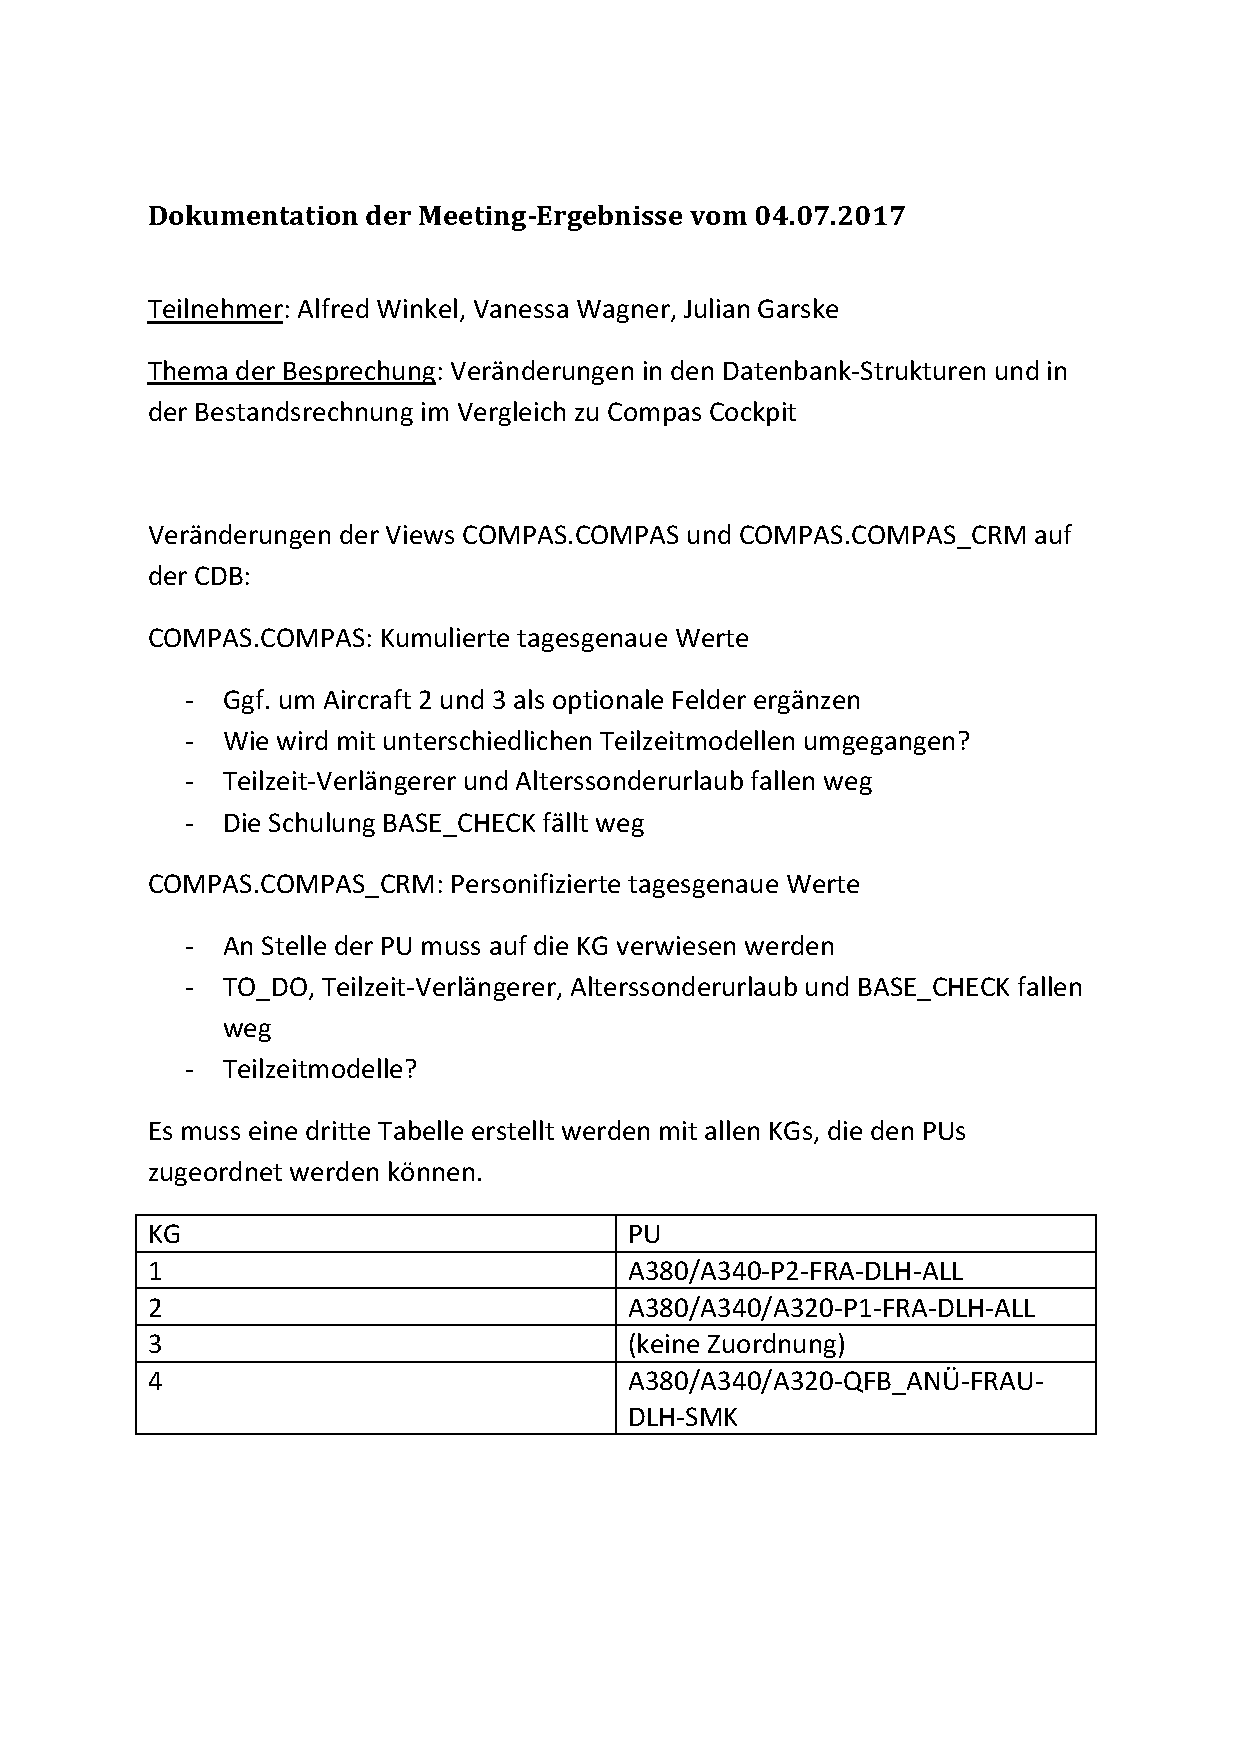
\includepdf[pages=1, pagecommand={\section{Gesprächsprotokoll vom 4. Juli 2017} \label{meeting0407}},  scale = 0.95]{Meeting0407.pdf}
\includepdf[pages=2-,pagecommand={}]{Meeting0407.pdf}


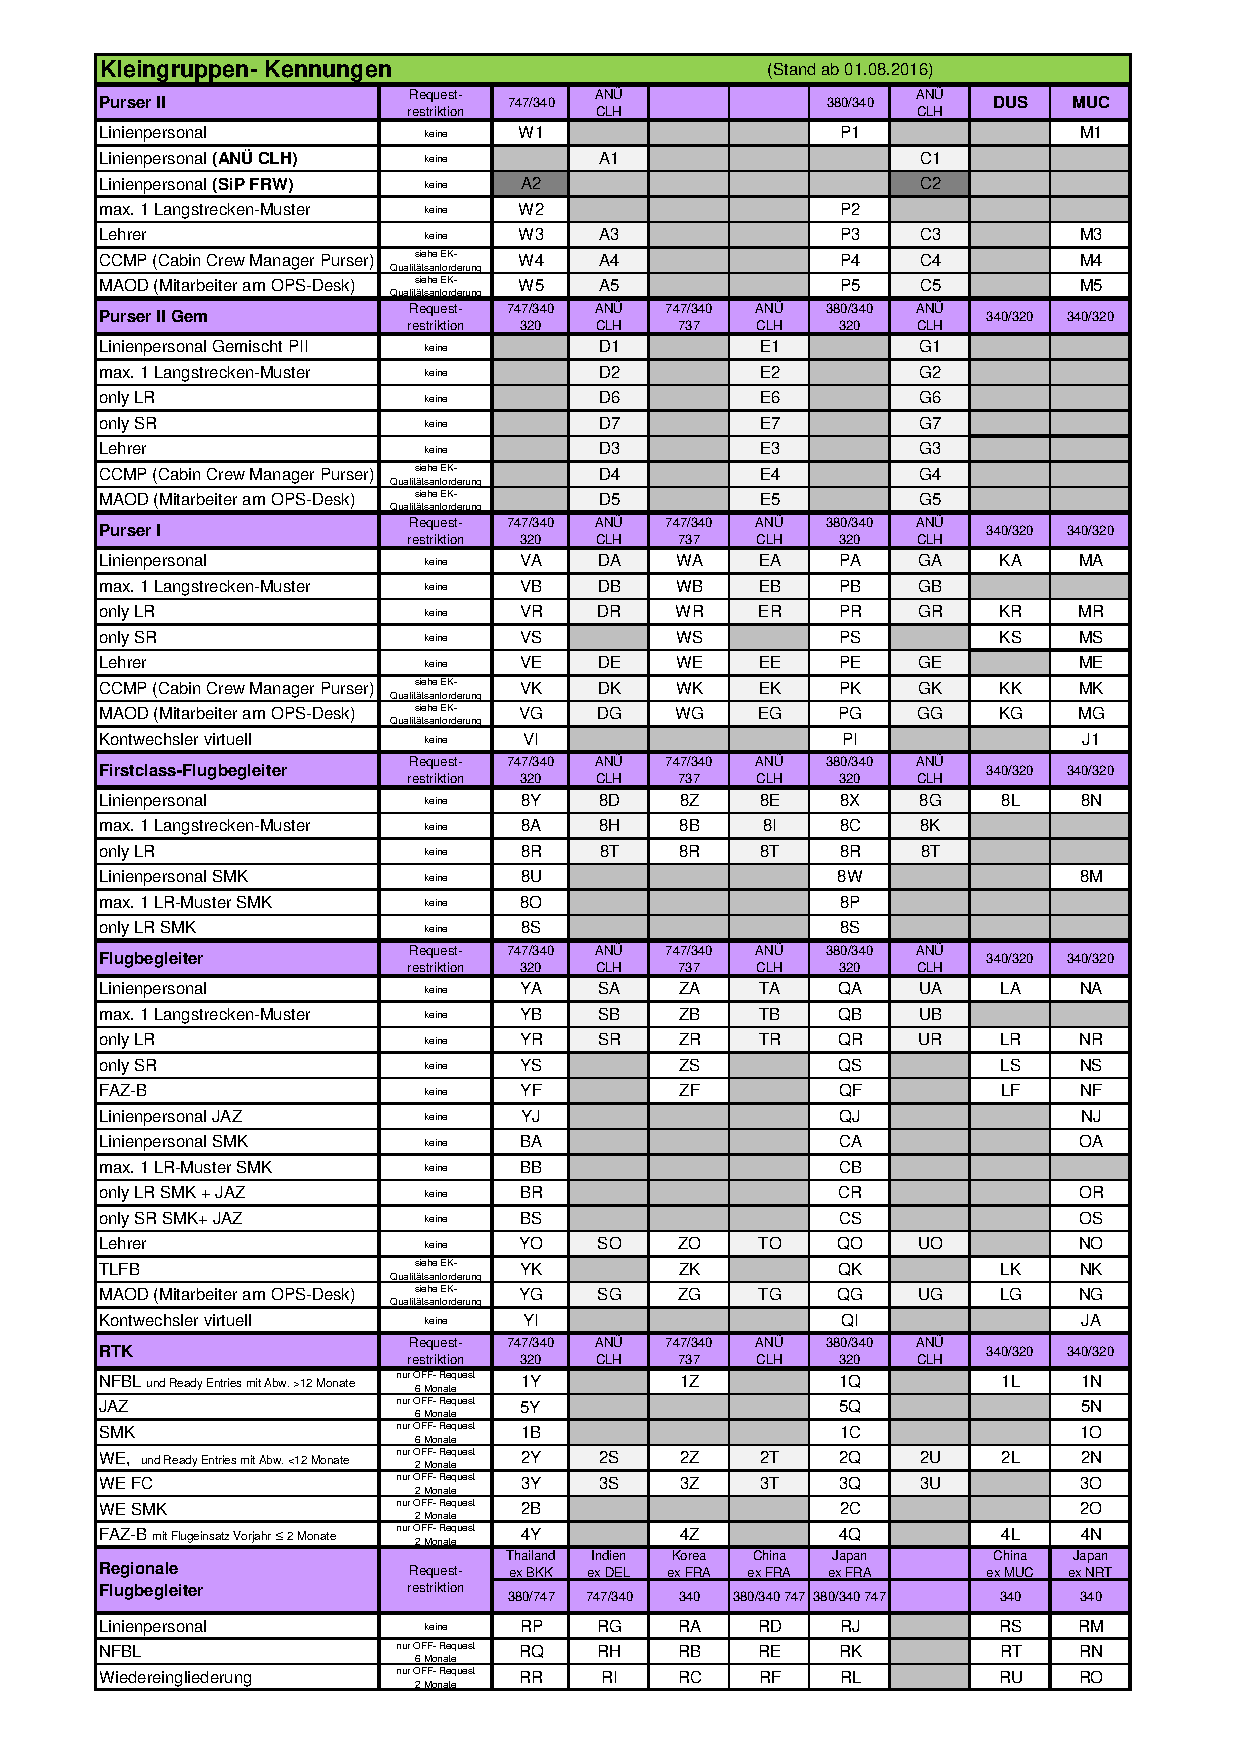
\includepdf[pagecommand={\section{Beispiele für Kleingruppen und Planungseinheiten} \label{kgpu}}, scale = 0.8, keepaspectratio]{Kleingruppen.pdf}
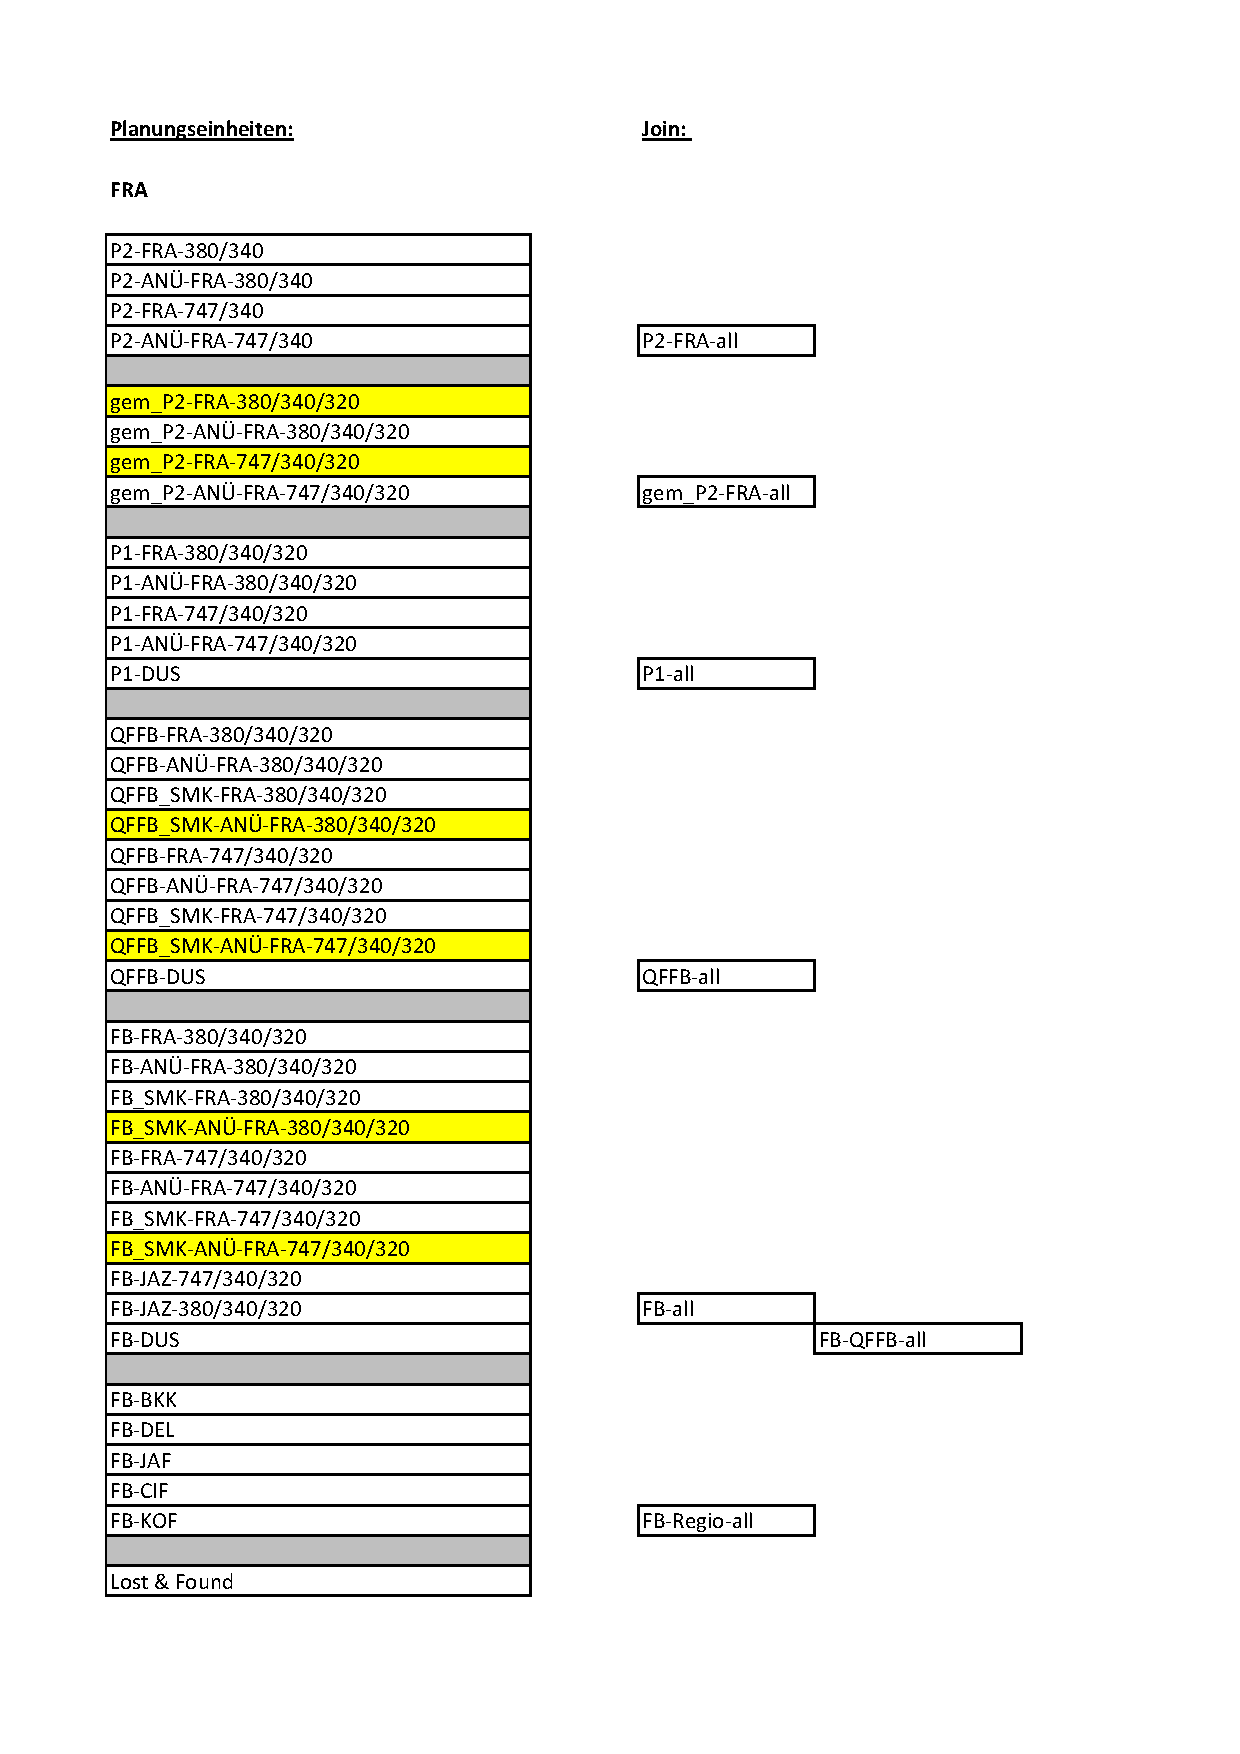
\includepdf{Planungseinheiten.pdf}

\newpage

\end{document}

